\documentclass{scrartcl}			% defines the kind of document you want to produce

% Include different packages:
\usepackage[utf8]{inputenc}
\usepackage[T1]{fontenc}
\usepackage{lmodern}
\usepackage[english]{babel}
\usepackage{amsmath}
\usepackage{float}
\usepackage{graphicx}           	% include graphics
\usepackage{caption}
\usepackage{subcaption}
\usepackage{hyperref}
\usepackage{listings}
\usepackage{fancyvrb}

\title{Neuroprothetik Exercise 6 \\\textsl{}
	Electric Stimulation}

\author{Aleksandra Teska}
\date{29. June 2018}


\begin{document} 					% Document begins here

\maketitle
\section{Calculate the Potential Field}
The goal of this exercise is calculating the potential at a distance r from a current point-source, that can be calculated by:
\begin{align}
\Phi = \frac{\rho}{4\pi} * \frac{I}{r}
\end{align}

\subsection{Potential Field}
Using the following parameters, plot the potential field for a 50 $\mu m$ by 50 $\mu m$ slice in a distance of 10 $\mu m$ from the point source. With parameters:\textit{ medium = 300 $\Omega cm$ , I = 1 mA}. The results can be seen in \ref{fig1}.

\subsection{Activation Function}
Calculate and plot 
a) the external potential ( \ref{fig21} )
b) the electric field (\ref{fig22})
c) the activation (\ref{fig23})
function along a 50 $\mu m$ peace of axon positioned 10 $\mu m$ from a current point source. Plot
the three graphs for a electrode current of 1 mA and for -1 mA


\section{Create a Neuron Model}
The exercised aimed to enhance the neuron model implemented in exercise 6, to now consider an the influence of an external potential. Given parameters were used: $\rho_{axon}$ = 0.01  $k \Omega cm$, $r_{axon}$ = 1.5 * $10^{ - 4} cm$,  $l_{comp}$ = 0.5 * $10^{ - 4} cm$, 

\subsection{Stimulate the Axon}
The following stimulation sequences were created and run with your axon positioned as in section. Run the simulation for about 30 ms and position your pulse at t=5 ms
\begin{enumerate}
	\item Stimulation by a mono-phasic current pulse, phase duration = 1 ms, current = -0.25 mA (\ref{fig31})
	\item Stimulation by a mono-phasic current pulse, phase duration = 1 ms, current = -1 mA (\ref{fig32})
	\item Stimulation by a bi-phasic current pulse (negative phase first), phase duration = 1 ms, amplitude = 0.5 mA (\ref{fig33})
	\item Stimulation by a bi-phasic current pulse (negative phase first), phase duration = 1 ms, amplitude = 2 mA (\ref{fig34})
	\item Stimulation by a mono-phasic current pulse, phase duration = 1 ms, current = 0.25 mA (\ref{fig35})
	\item Stimulation by a mono-phasic current pulse, phase duration = 1 ms, current = 5 mA (\ref{fig36})
\end{enumerate}

\subsection{Interpretation of the result}
\begin{enumerate}
\item Mono-phasic current pulse of -0.25 mA caused an external field outside of the multi-compartment model. The neurons between 40 and 60 got excited, but the change in their potentials did not elicit a spike. The shape (amount of compartments that were influenced by the external field (\ref{fig21}) can be explained by the distance from the spike on 50 element on the axon. We can also notice dark blue spots, indicating decreasing voltage.
\item Mono-phasic current pulse of -1mA also caused a change of compartments potential and then elicit spikes on the close neurons, that later on propagated through the model. The potential went up to around 100 mV, indicating spiking(\ref{fig32}). Two spike trains can be explained by the shape of the activation function (\ref{fig23}).
\item Stimulation with bi-phasic action potential of amplitude -0.5mA did not cause the spike. Impulse of the potential has to integrate to the specific size to cause excitation of the neurons. Due to bi-phasic type of the stimulation, the shape caused by the Ve is different.
\item Bi-phasic current of 2mA cause same behavior as in the experiment 2.
\item Application of small mono-phasic positive pulse of 0.25 mA caused slight hyper-polarization (decreased potential) of the compartments influenced by it (opposite to (\ref{fig31}).
\item Monophonic pulse of 5mA caused voltage drop around compartments 40 to 60 (up to -25mV). 
As in other experiments, around the main point of stimulation the opposite voltage filed appeared (dark blue parts in (\ref{fig31}). In this case went positive and above the threshold. Electric field caused activation of further compartments and action potentials propagating through the corresponding compartments.
\end{enumerate}
\newpage
\section{Plots}

%\subsection{Exercise 1}
\begin{figure}[hbpt!]					%start figure-environment
	\begin{flushleft}
		%\hspace*{-0.3in}
		\centering
		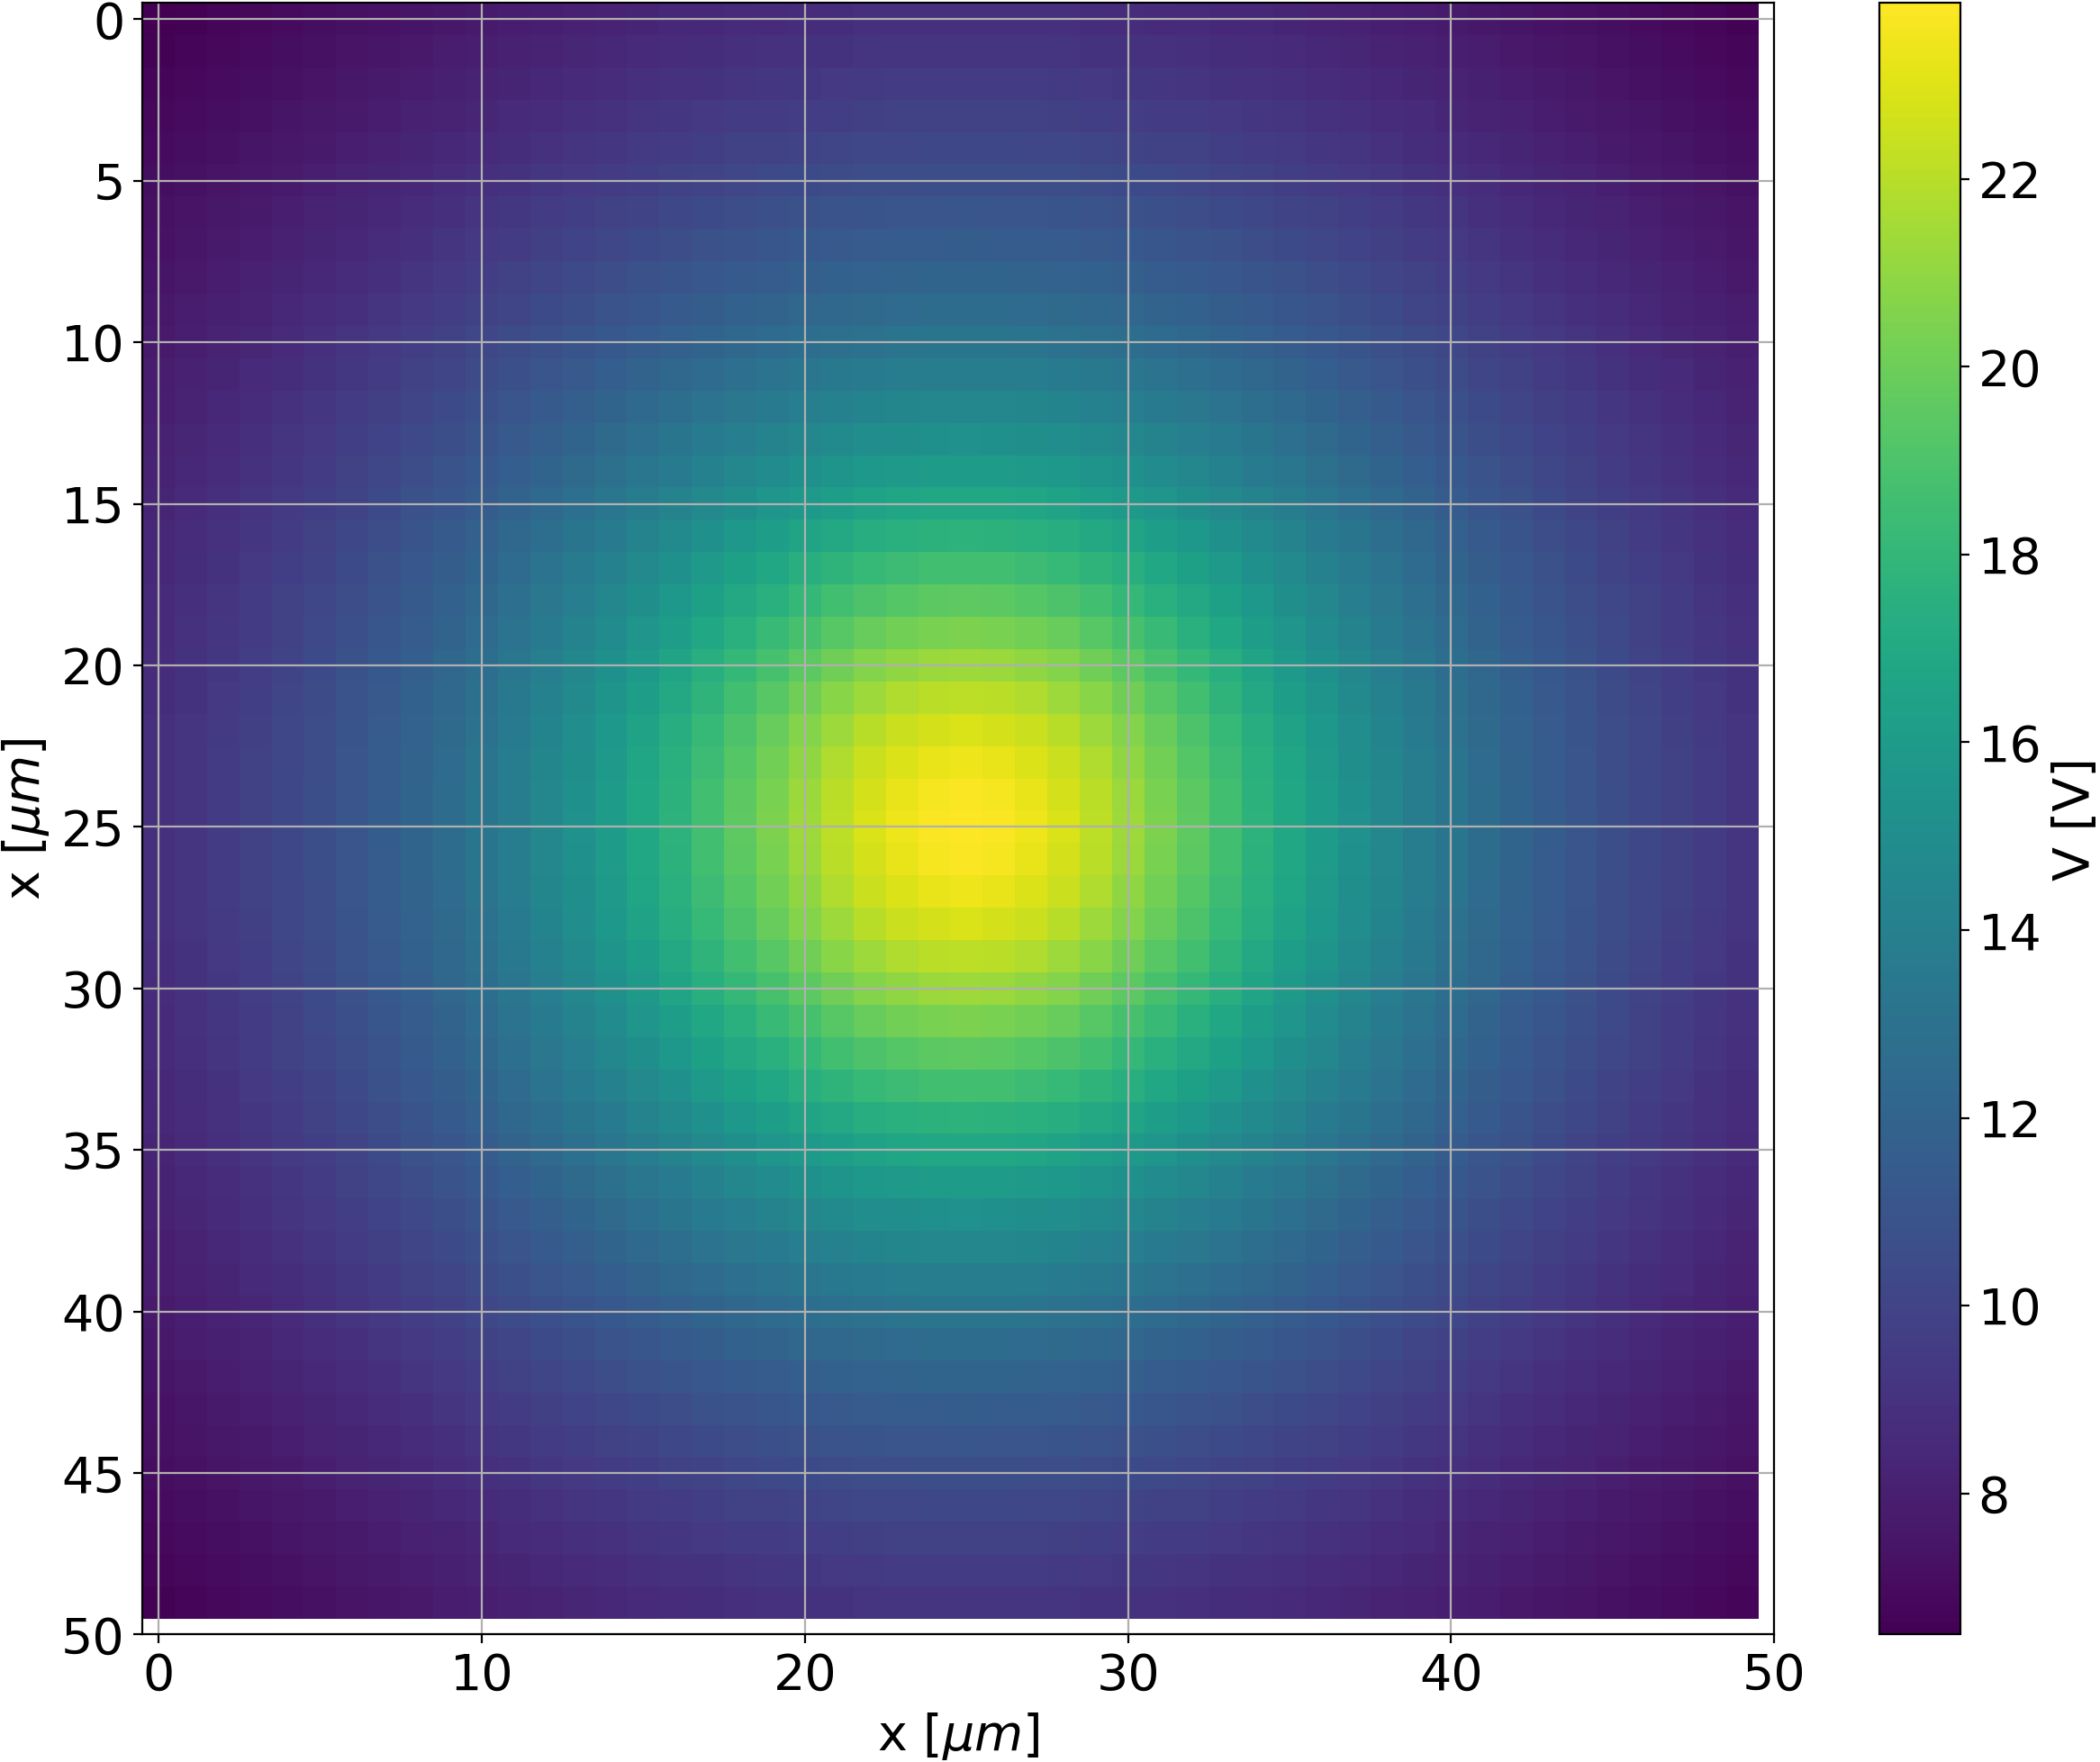
\includegraphics[scale=0.35]{1.png}
		\captionsetup{width=\linewidth}  %choose the with of the caption
		\caption{The potential field for a 50$\mu m$ by 50$\mu m$ slice in a distance of 10$\mu m$ from the point source.}		
		\label{fig1} %choose a label, see subsection references
	\end{flushleft}
\end{figure}

\begin{figure}[hbpt!]					%start figure-environment
	 \begin{flushleft}
		\hspace*{-0.3in}
		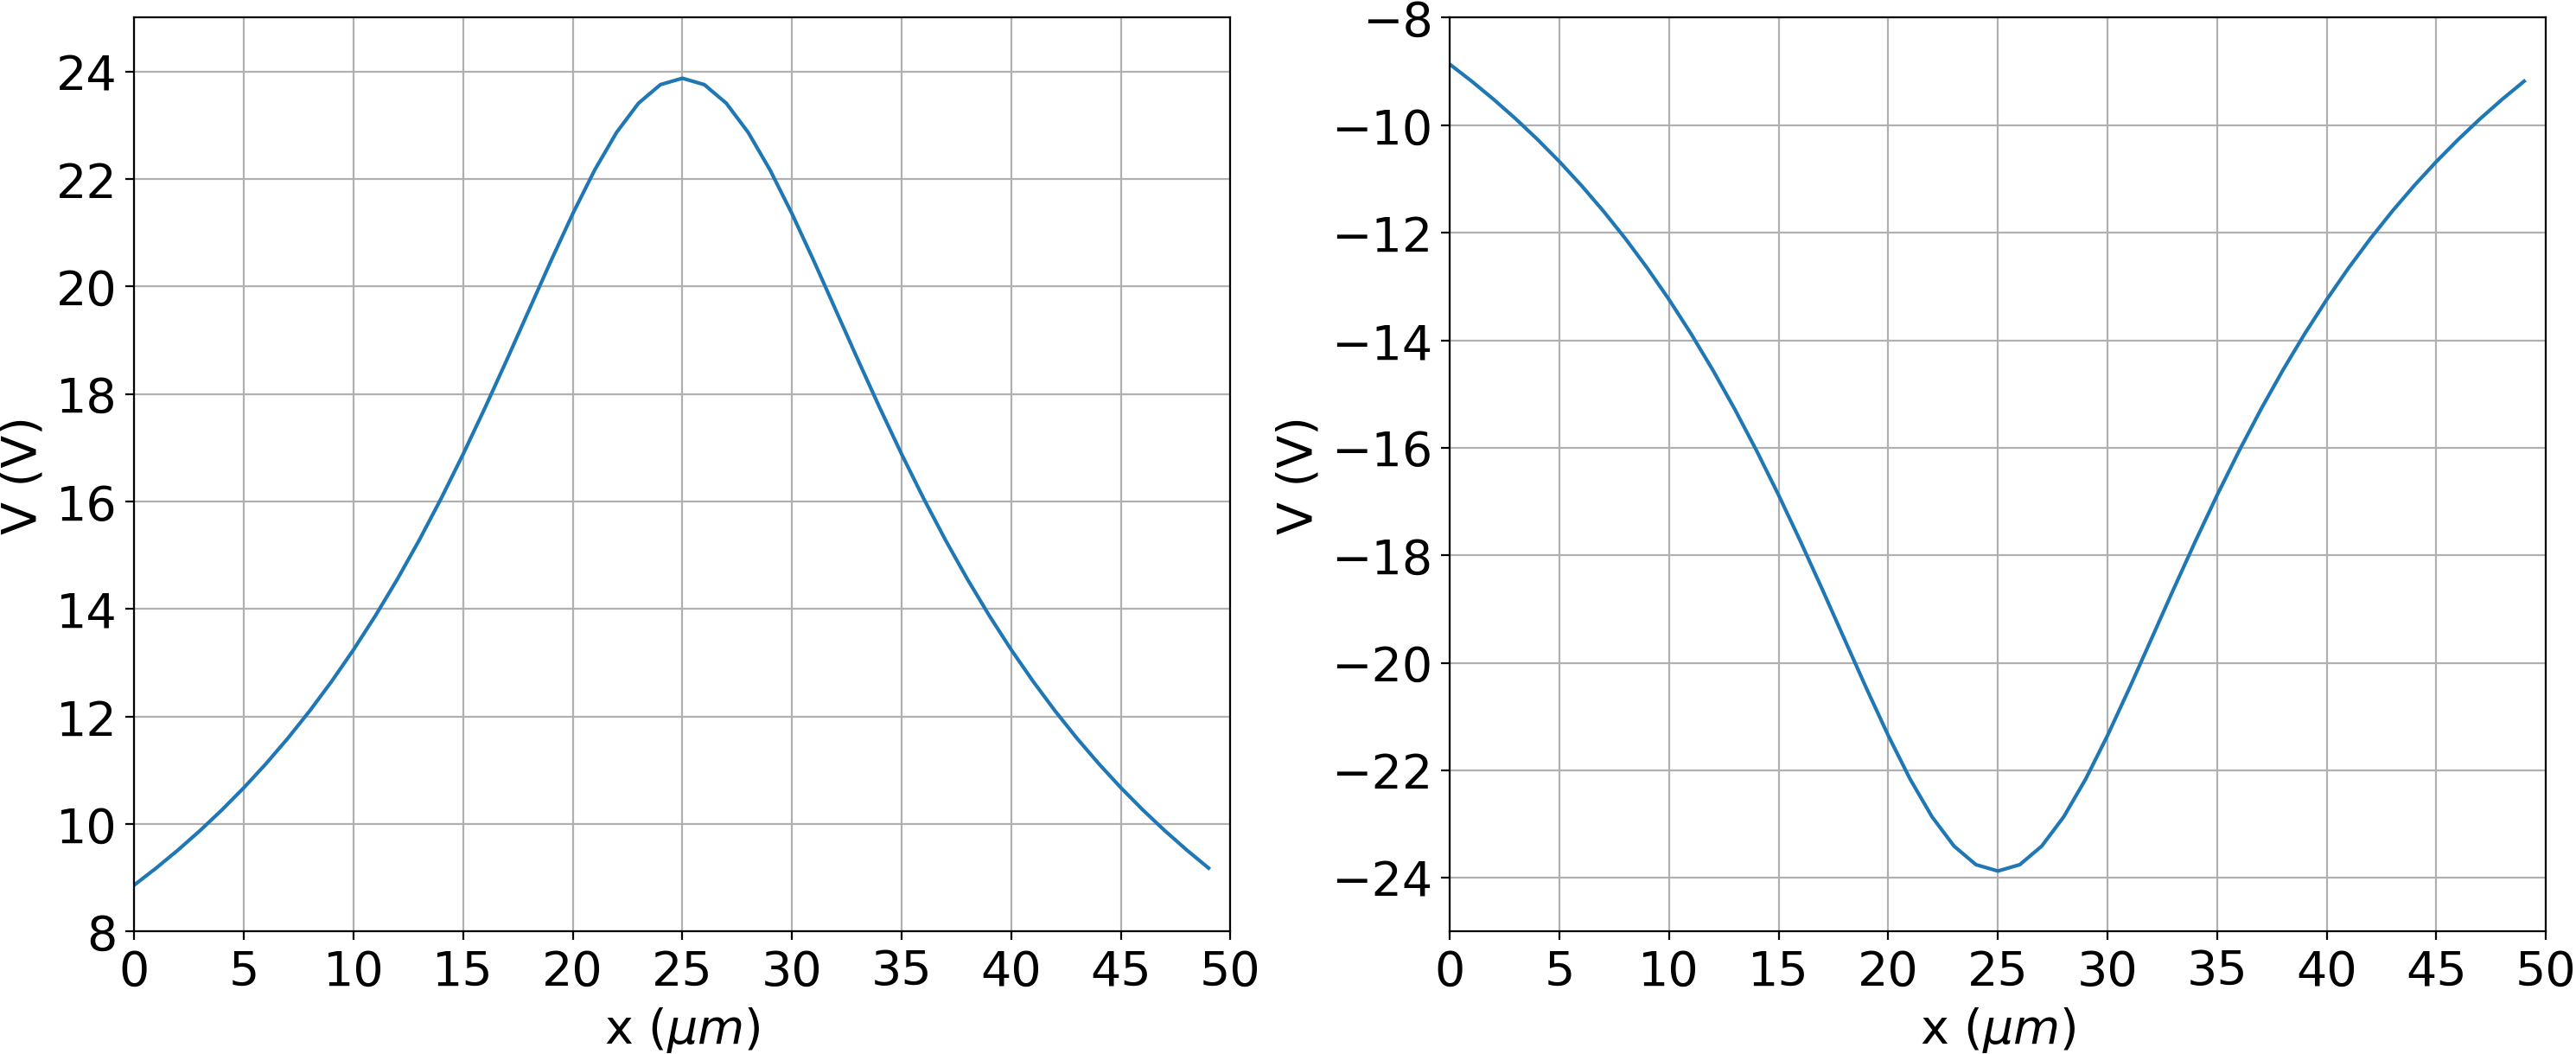
\includegraphics[scale=0.4]{2_1.png}
		\captionsetup{width=\linewidth}  %choose the with of the caption
		\caption{The external potential along a 50$\mu m$ peace of axon positioned 10$\mu m$ from a current point source.}
		\label{fig21} %choose a label, see subsection references
	\end{flushleft}
\end{figure}

\begin{figure}[hbpt!]					%start figure-environment
	\begin{flushleft}
		\hspace*{-0.3in}
		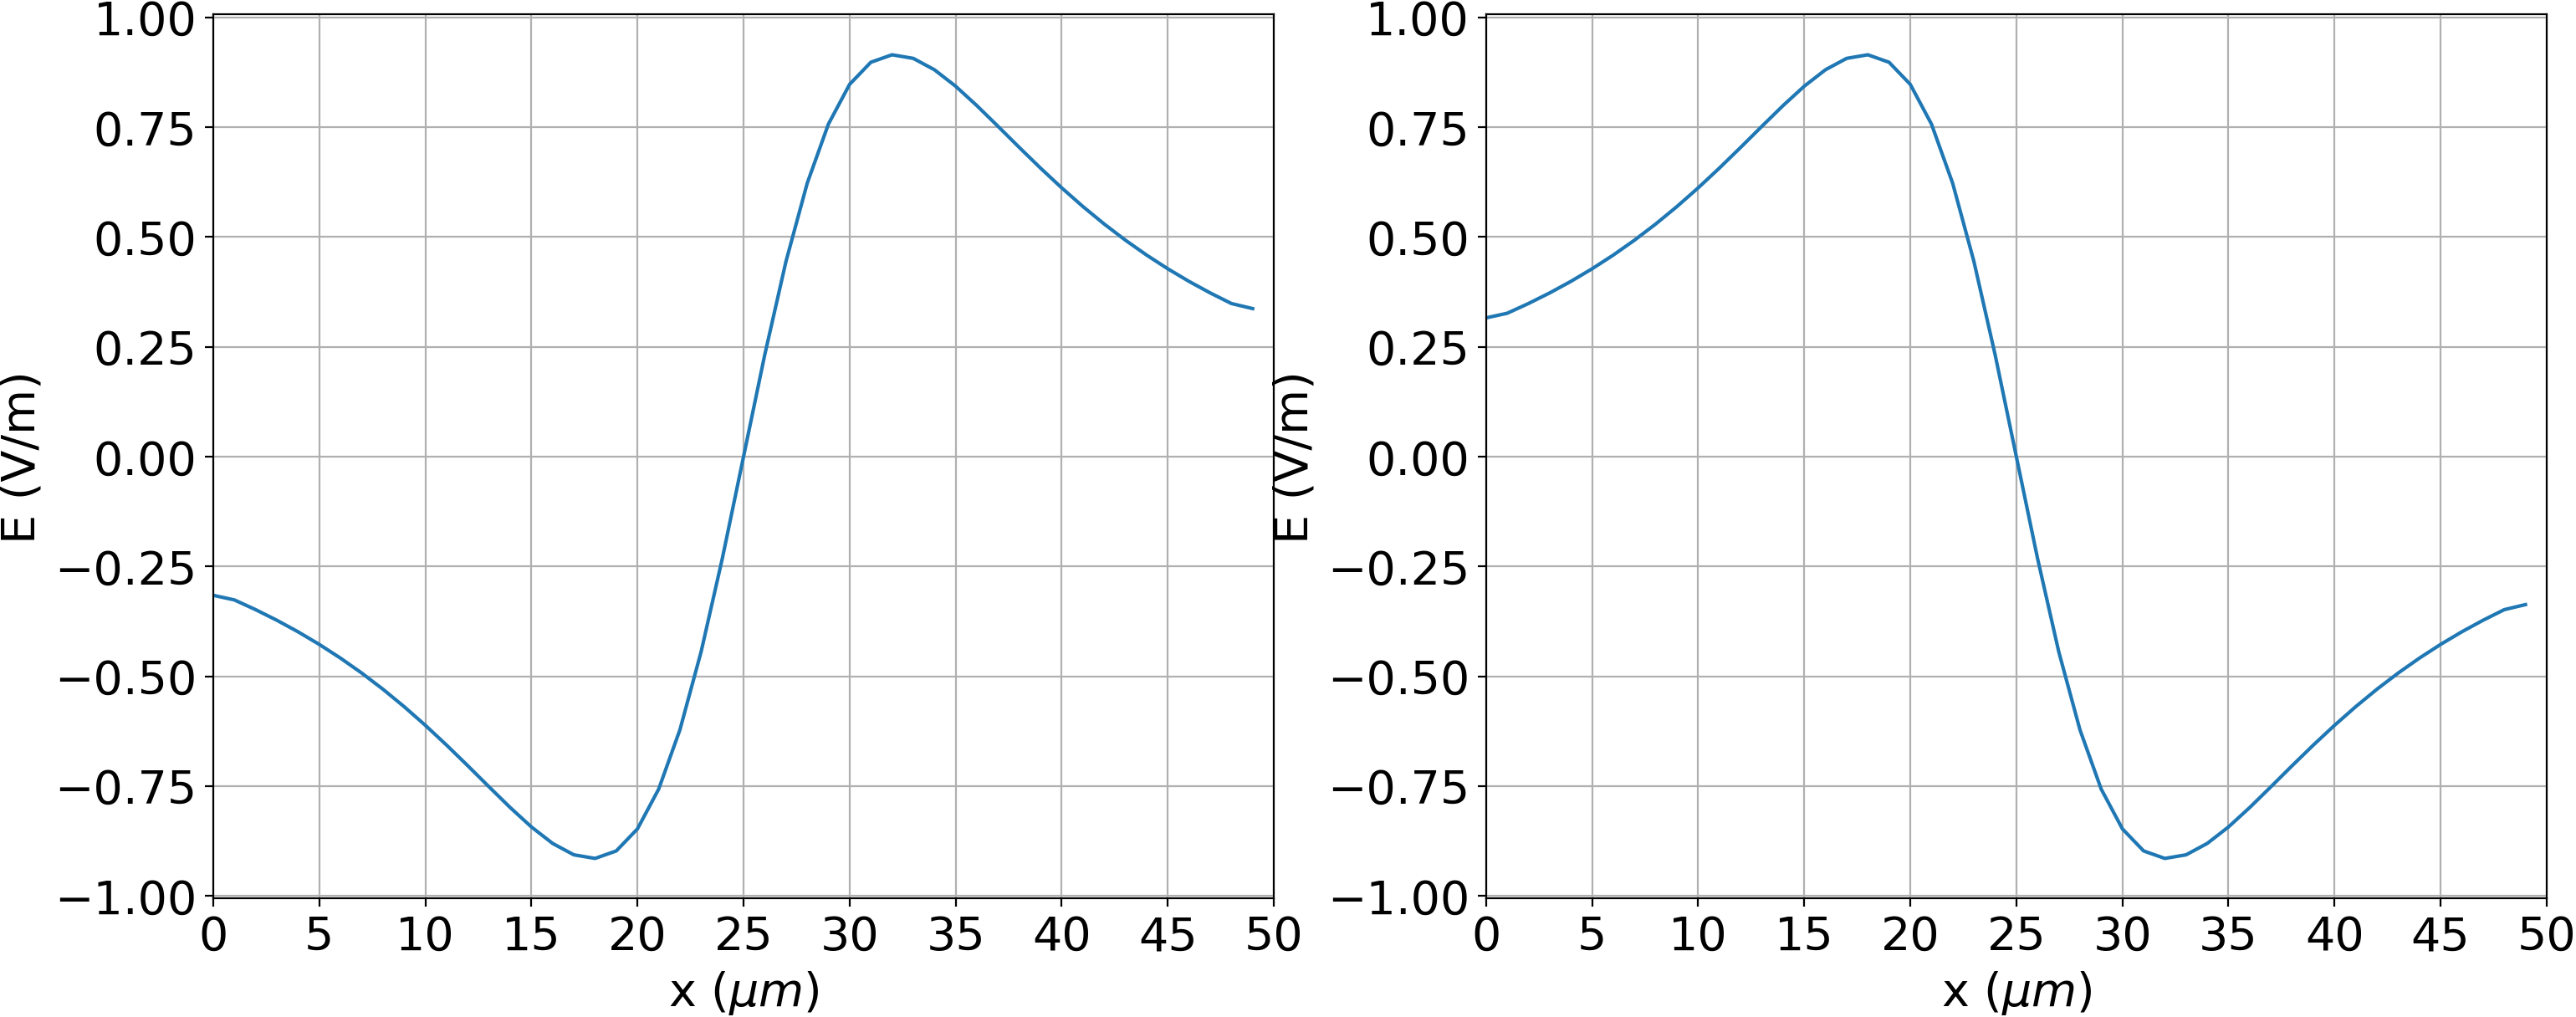
\includegraphics[scale=0.41]{2_2.png}
		\captionsetup{width=\linewidth}  %choose the with of the caption
		\caption{The electric field along a 50$\mu m$ peace of axon positioned 10$\mu m$ from a current point source.}		
		\label{fig22} %choose a label, see subsection references
	\end{flushleft}
\end{figure}

\begin{figure}[hbpt!]					%start figure-environment
	\begin{flushleft}
		\hspace*{-0.3in}
		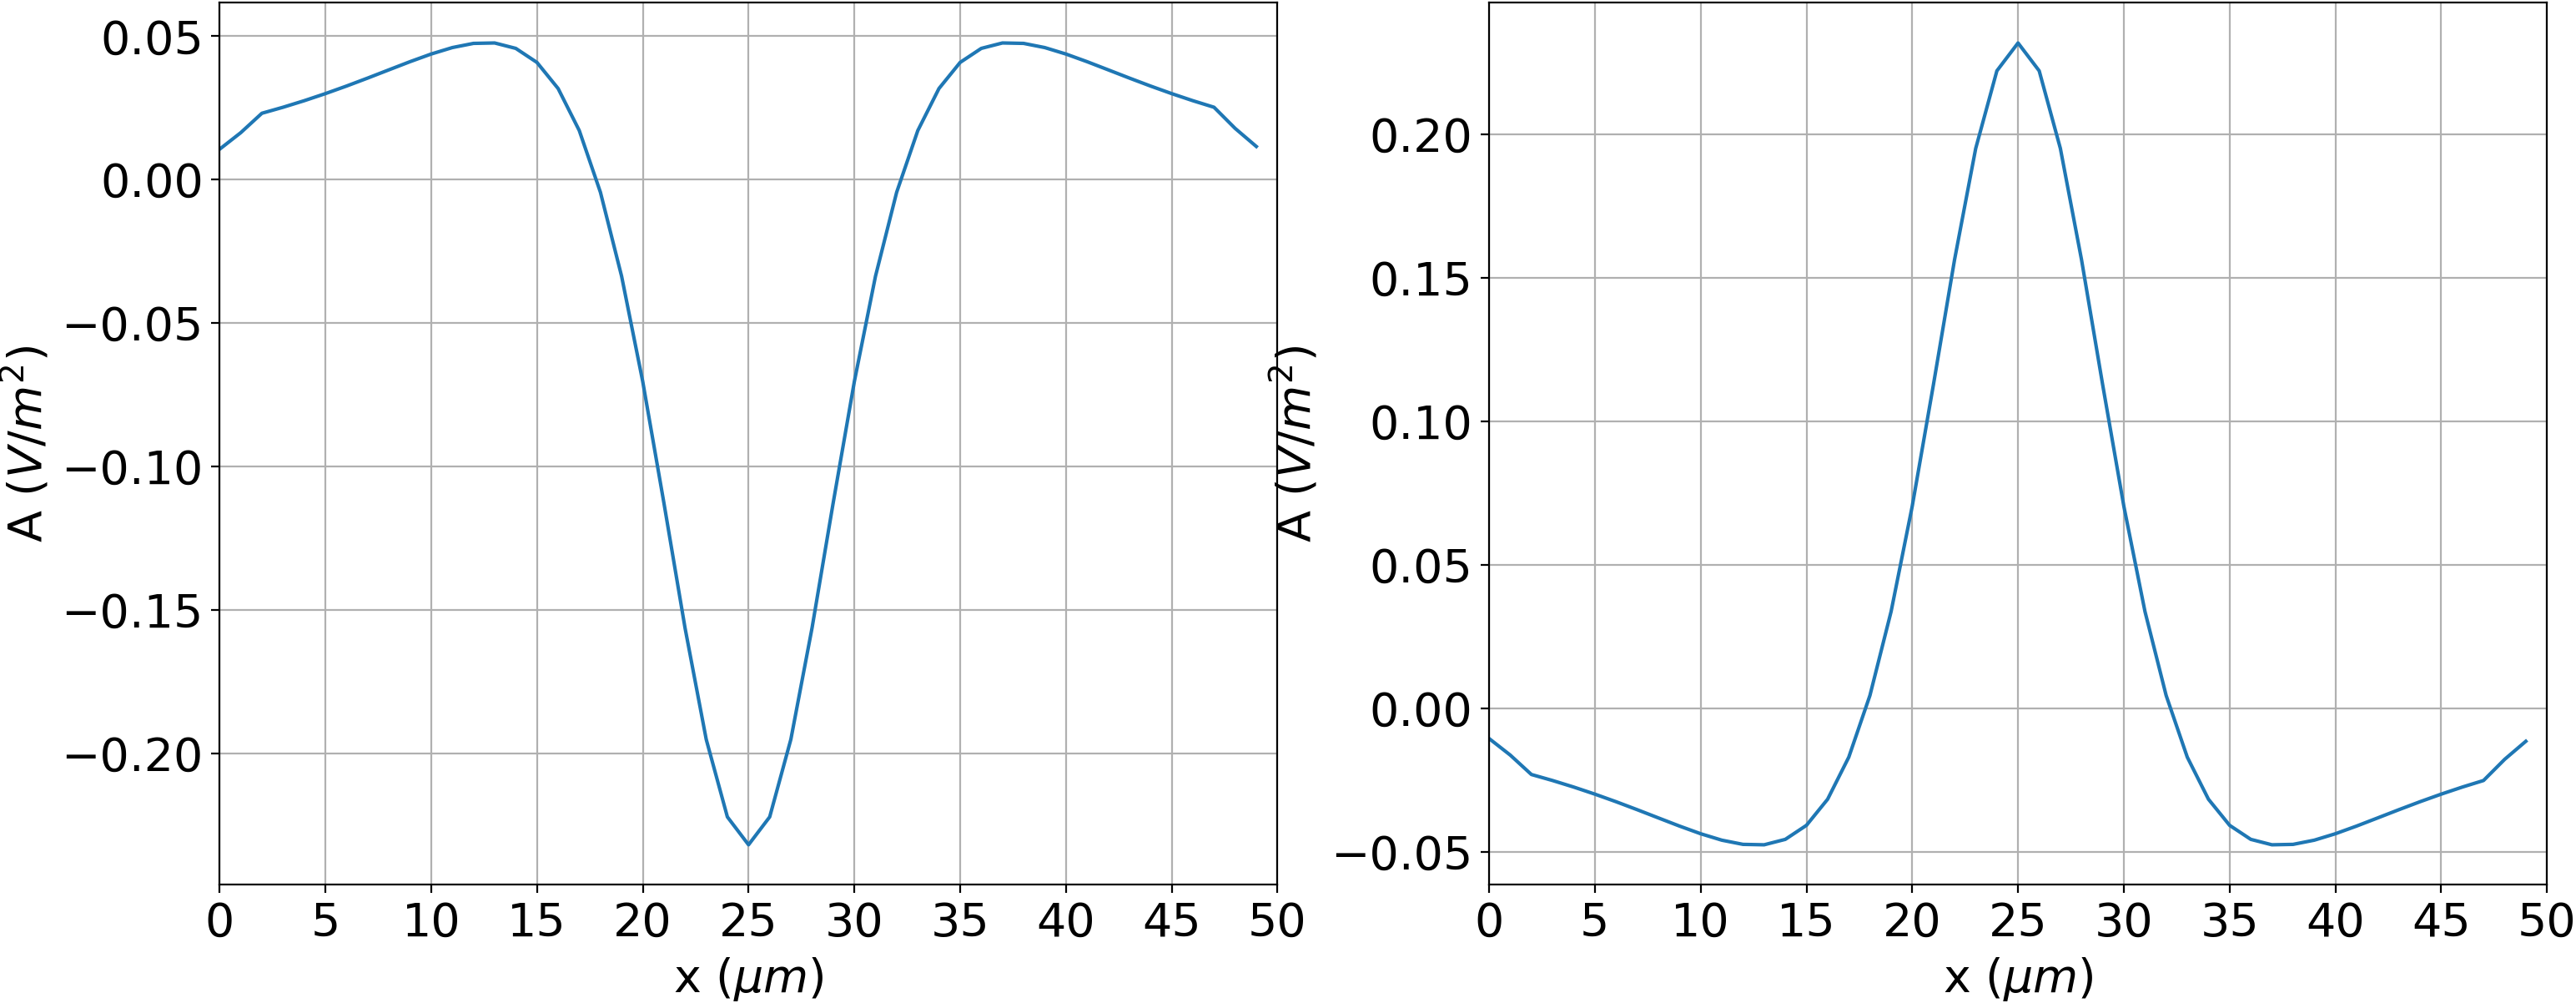
\includegraphics[scale=0.41]{2_3.png}
		\captionsetup{width=\linewidth}  %choose the with of the caption
		\caption{The activation function along a 50$\mu m$ peace of axon positioned 10$\mu m$ from a current point source.}		
		\label{fig23} %choose a label, see subsection references
	\end{flushleft}
\end{figure}

\newpage
\subsection{Exercise 2}
\begin{figure}[hbpt!]					%start figure-environment
	\begin{flushleft}
		\hspace*{-0.3in}
		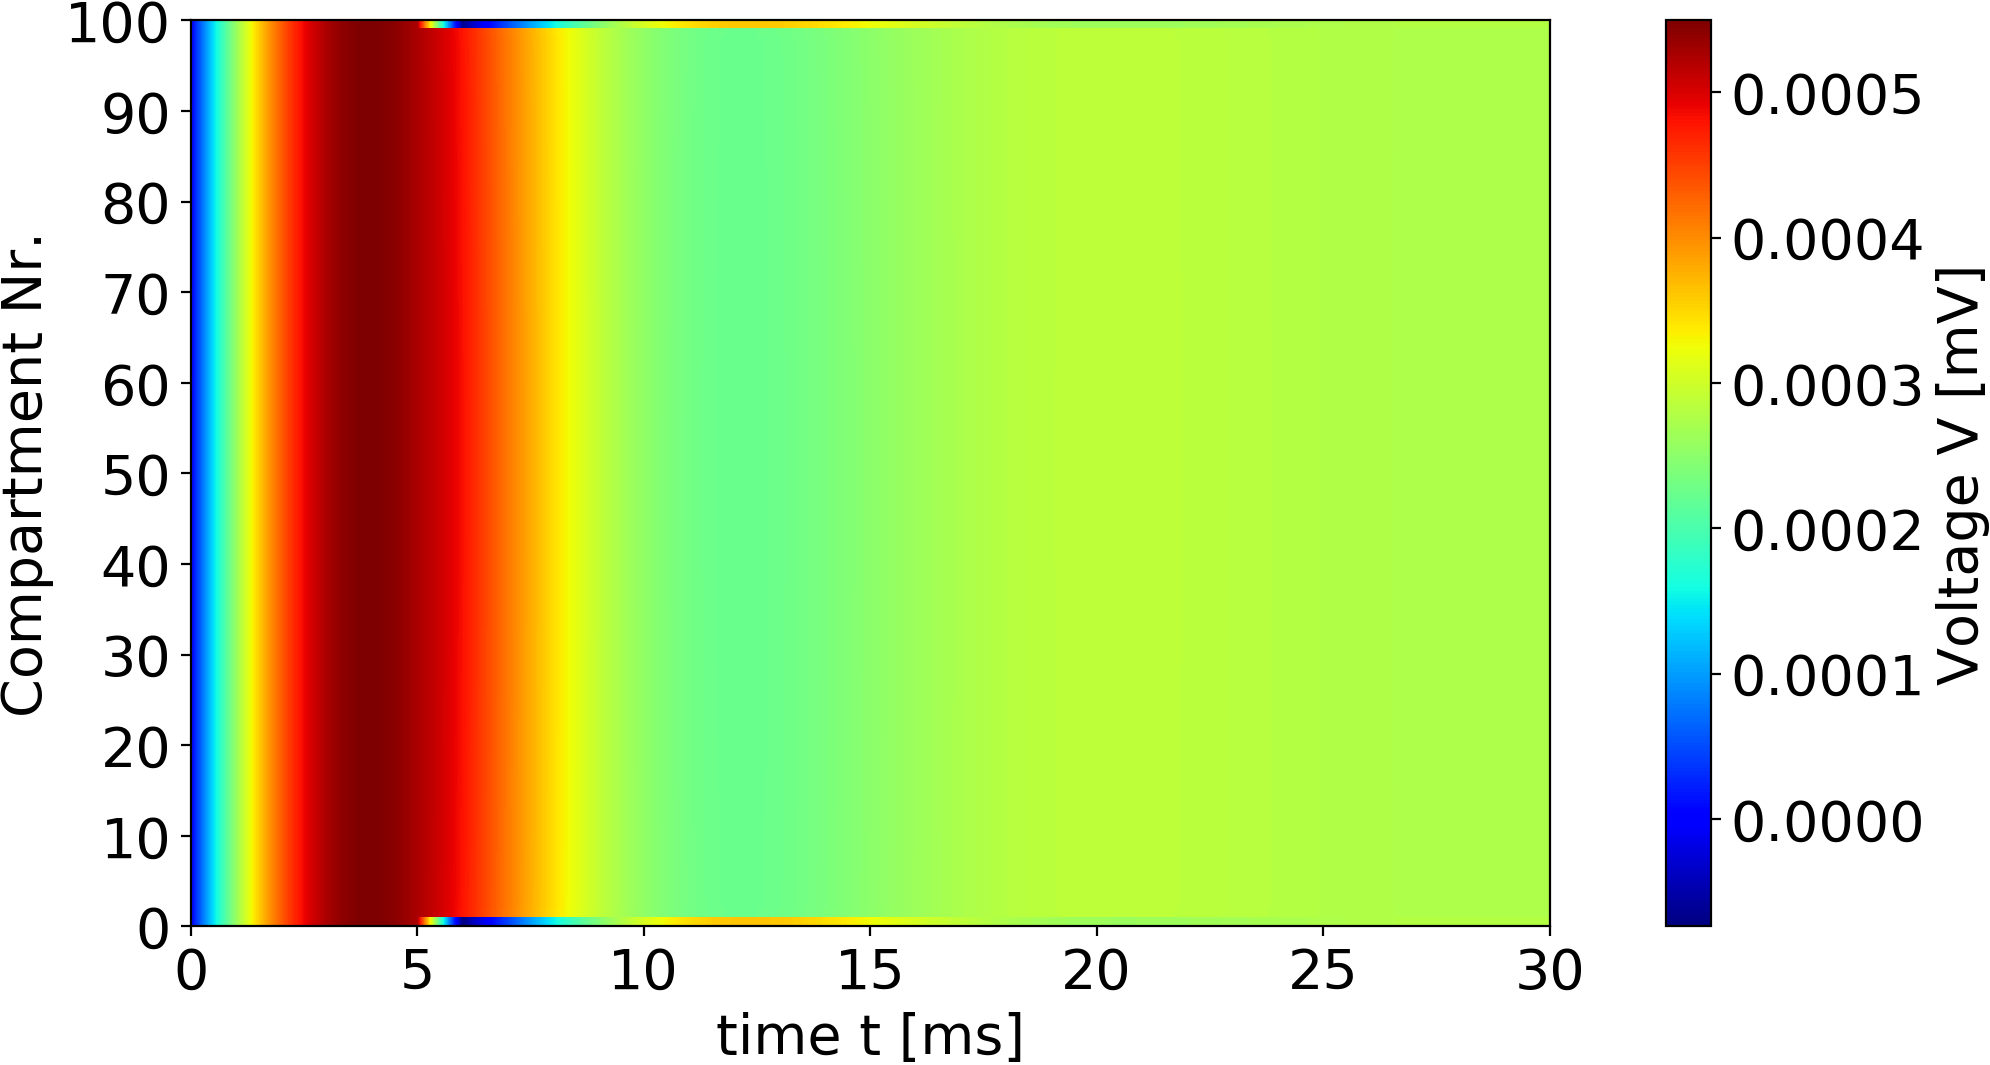
\includegraphics[scale=0.47]{3_1.png}
		\captionsetup{width=\linewidth}  %choose the with of the caption
		\caption{ Propagation of the action potential when stimulated at t = 5 ms with a phase duration of 1 ms. Additionally parameter: mono-phasic pulse	with -0.25 mA.}
		\label{fig31} %choose a label, see subsection references
	\end{flushleft}
\end{figure}
\begin{figure}[hbpt!]					%start figure-environment
	\begin{flushleft}
		\hspace*{-0.3in}
		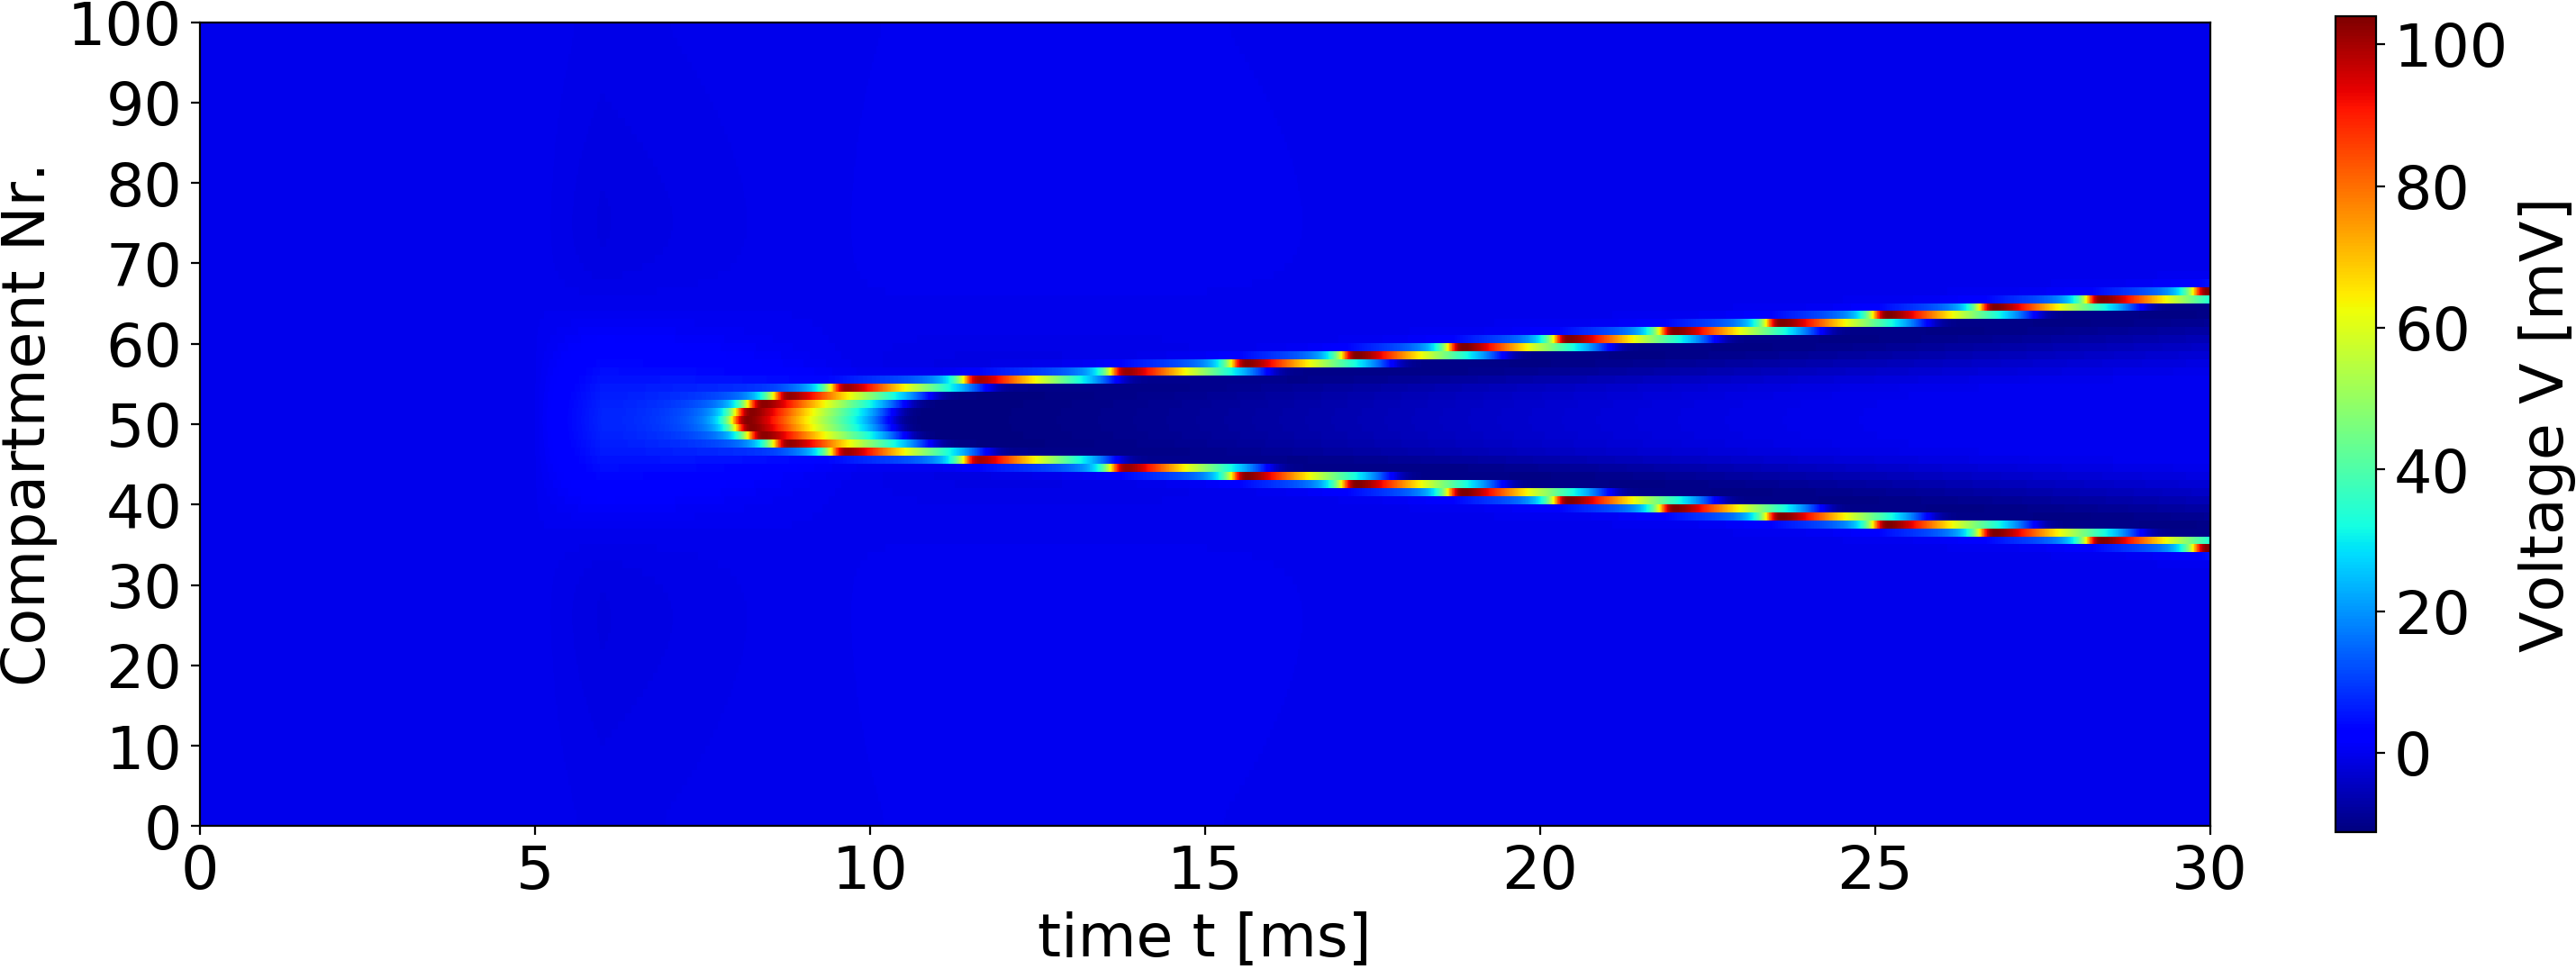
\includegraphics[scale=0.47]{3_2.png}
		\captionsetup{width=\linewidth}  %choose the with of the caption
		\caption{Propagation of the action potential when stimulated at t = 5 ms with a phase duration of 1 ms. Additionally parameter: mono-phasic pulse with -1 mA.}		
		\label{fig32} %choose a label, see subsection references
	\end{flushleft}
\end{figure}
\begin{figure}[hbpt!]					%start figure-environment
	\begin{flushleft}
		\hspace*{-0.3in}
		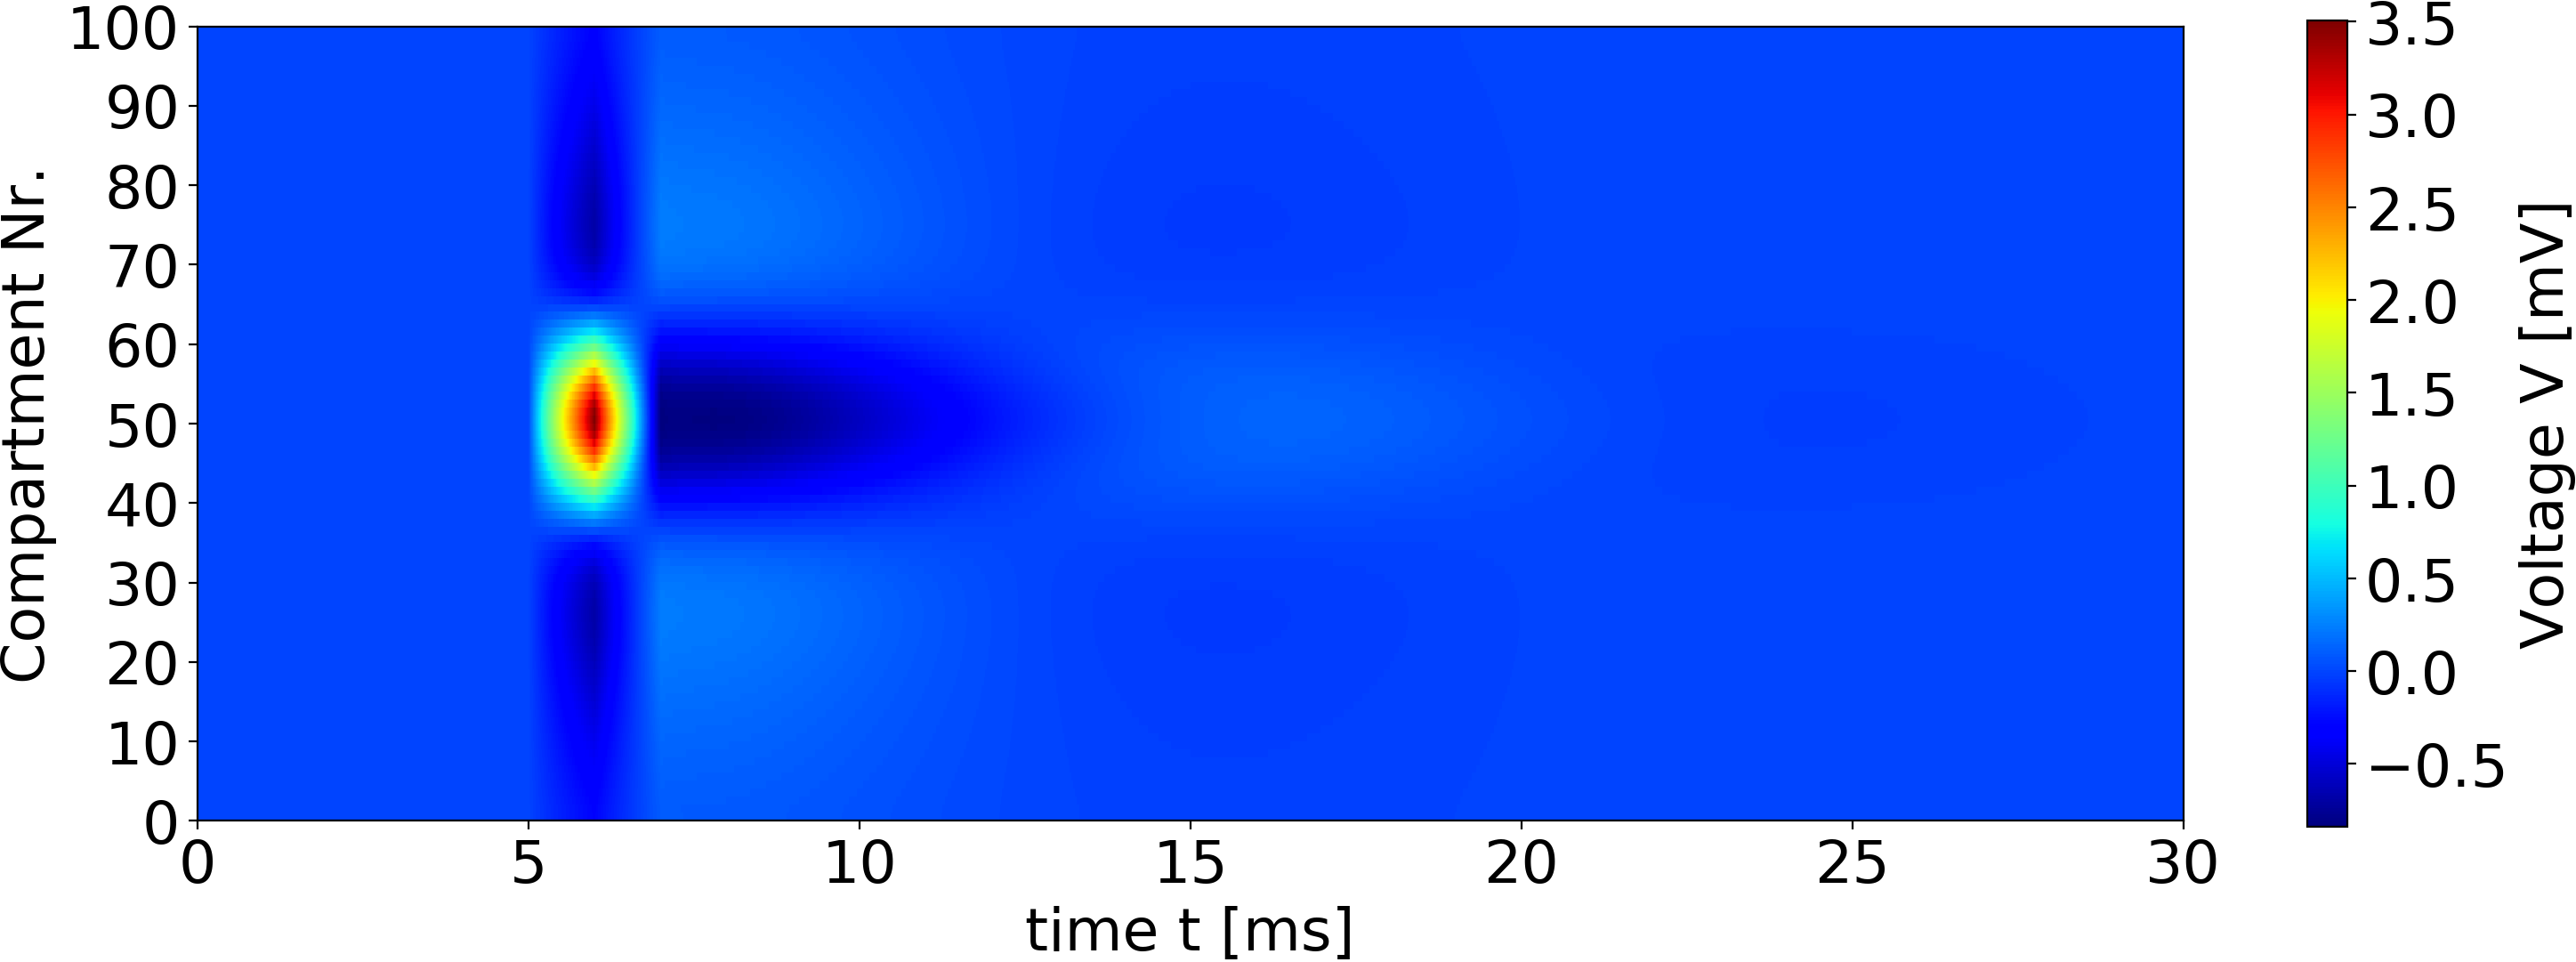
\includegraphics[scale=0.47]{3_3.png}
		\captionsetup{width=\linewidth}  %choose the with of the caption
		\caption{ Propagation of the action potential when stimulated at t = 5 ms with a phase duration of 1 ms. Additionally parameter: bi-phasic pulse with 0.5 mA.}		
		\label{fig33} %choose a label, see subsection references
	\end{flushleft}
\end{figure}
\begin{figure}[hbpt!]					%start figure-environment
	\begin{flushleft}
		\hspace*{-0.3in}
		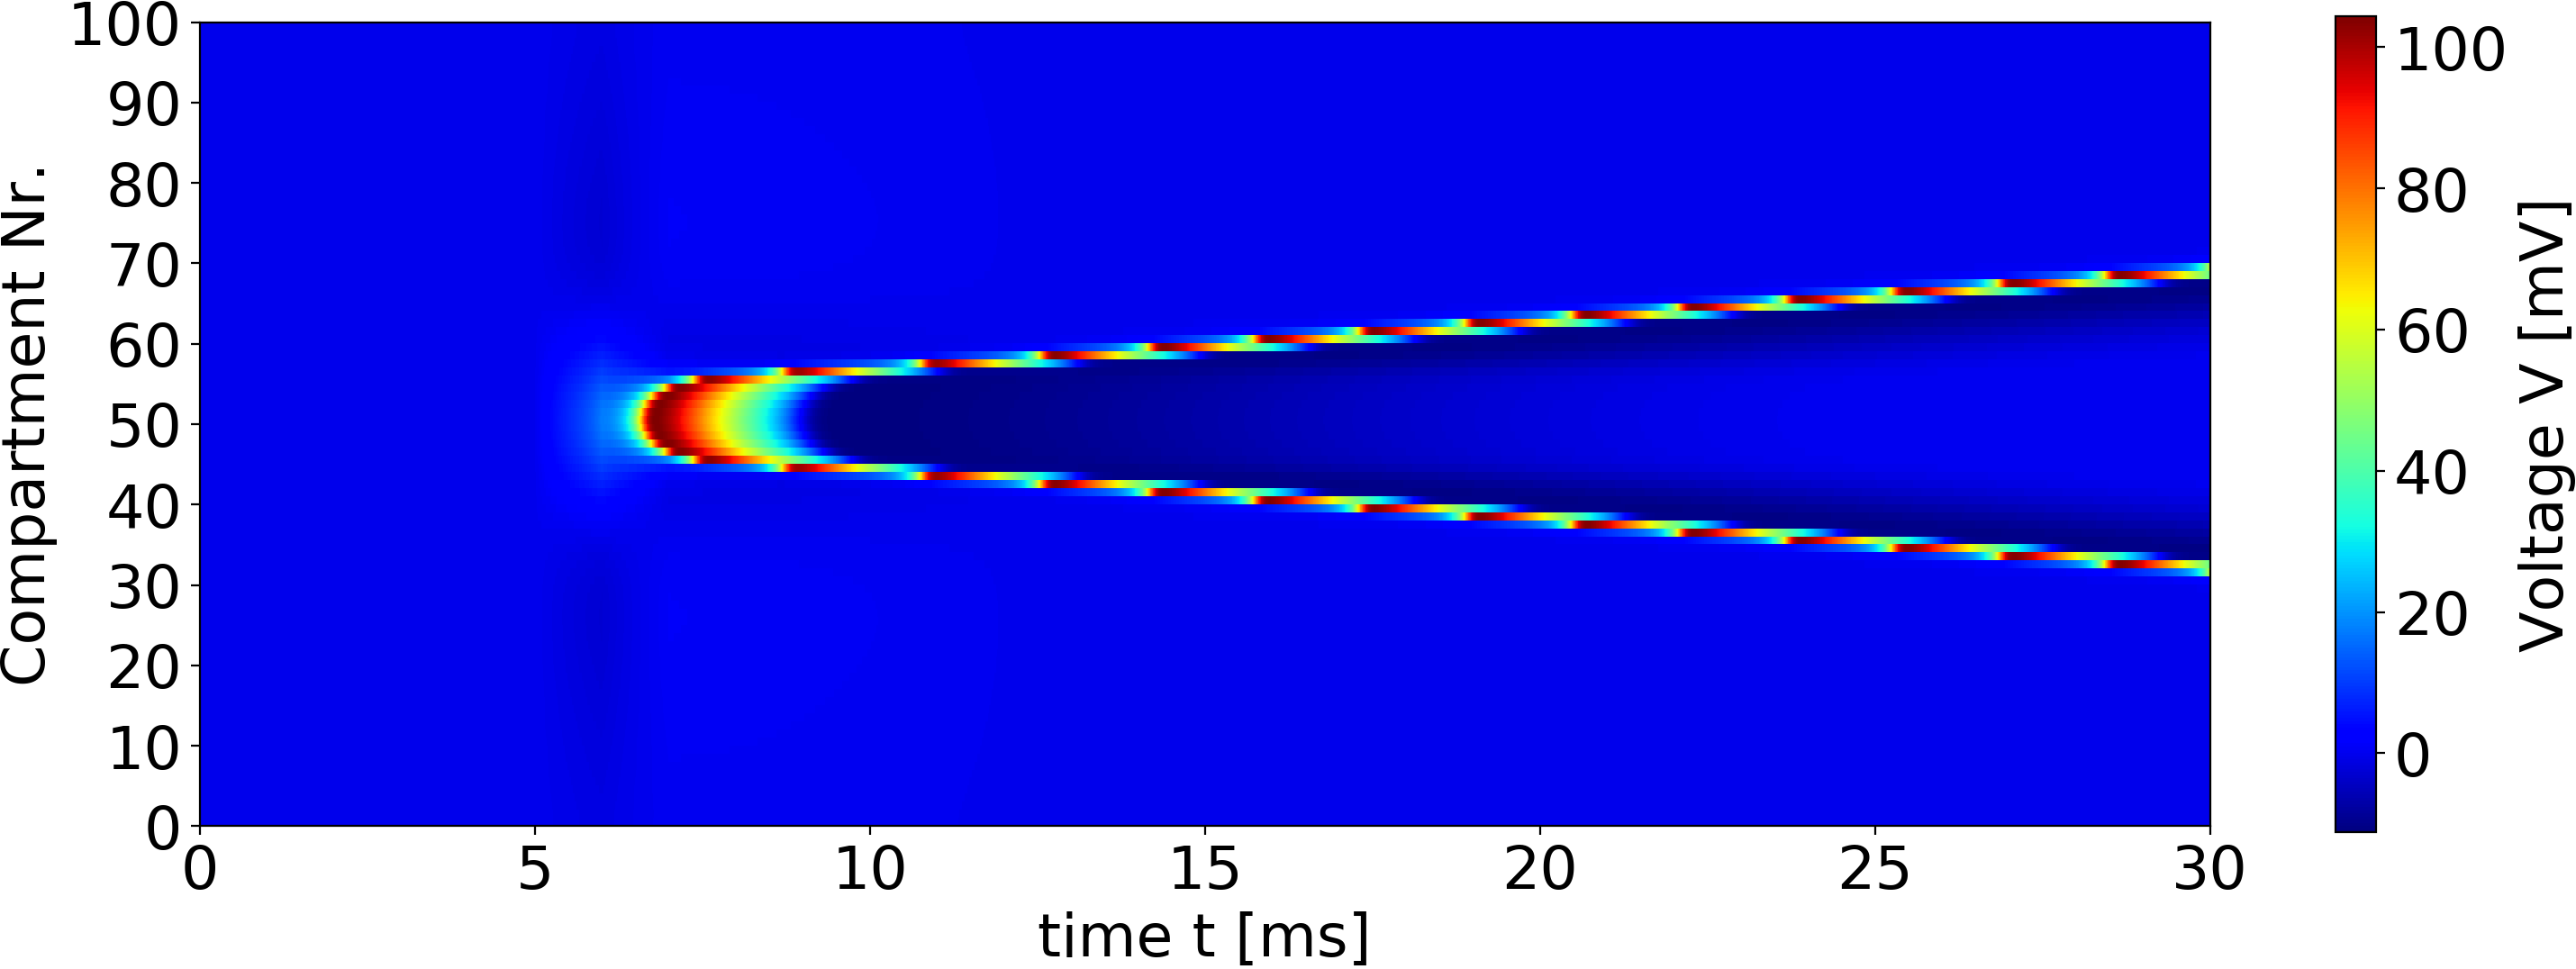
\includegraphics[scale=0.47]{3_4.png}
		\captionsetup{width=\linewidth}  %choose the with of the caption
		\caption{Propagation of the action potential when stimulated at t = 5 ms with a phase duration of 1 ms. Additionally parameter: bi-phasic pulse with 2 mA.}		
		\label{fig34} %choose a label, see subsection references
	\end{flushleft}
\end{figure}
\begin{figure}[hbpt!]					%start figure-environment
	\begin{flushleft}
		\hspace*{-0.3in}
		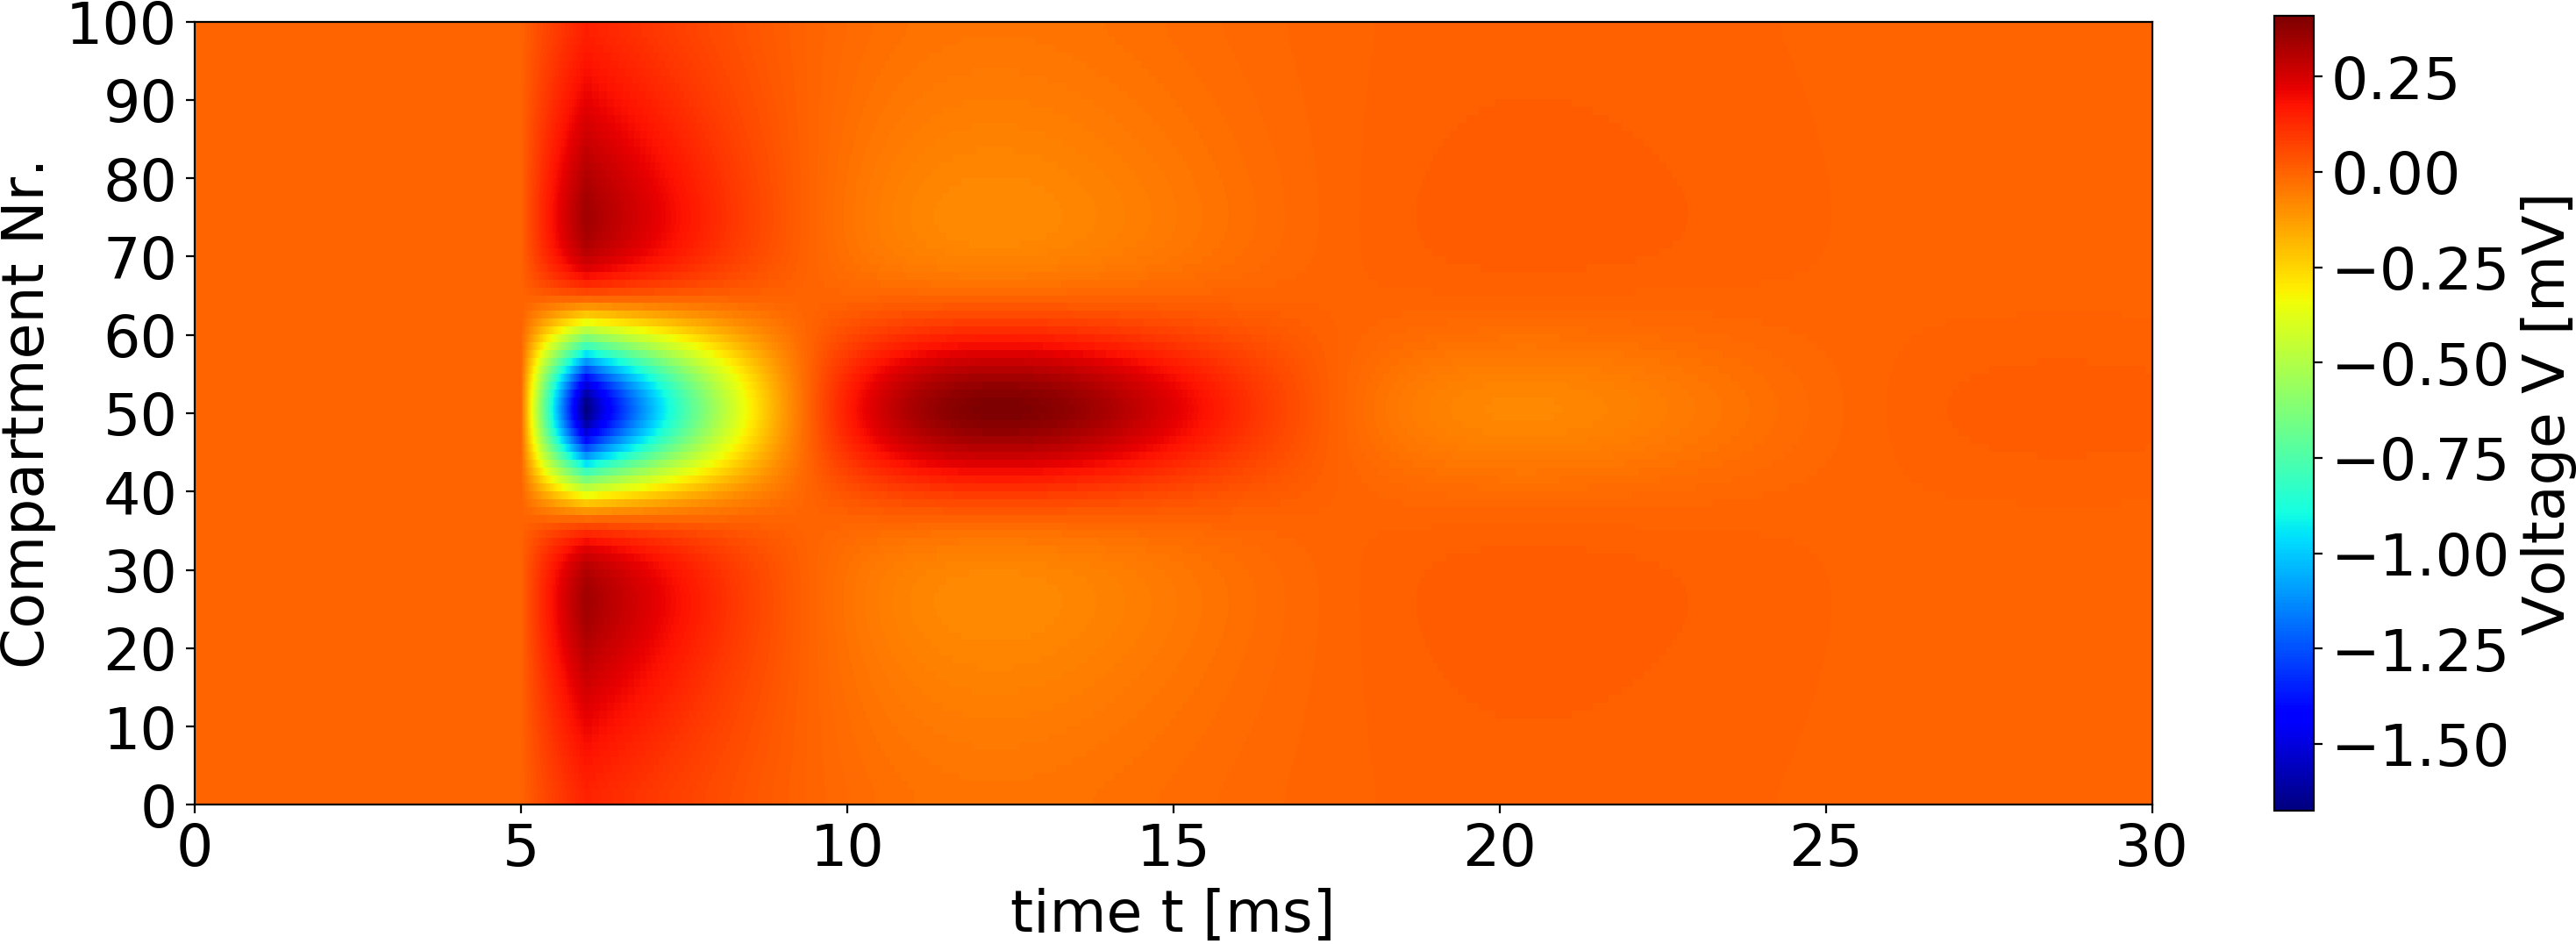
\includegraphics[scale=0.47]{3_5.png}
		\captionsetup{width=\linewidth}  %choose the with of the caption
		\caption{Propagation of the action potential when stimulated at t = 5 ms with a phase duration of 1 ms. Additionally parameter: mono-phasic pulse with 0.25 mA.}		
		\label{fig35} %choose a label, see subsection references
	\end{flushleft}
\end{figure}
\begin{figure}[hbpt!]					%start figure-environment
	\begin{flushleft}
		\hspace*{-0.3in}
		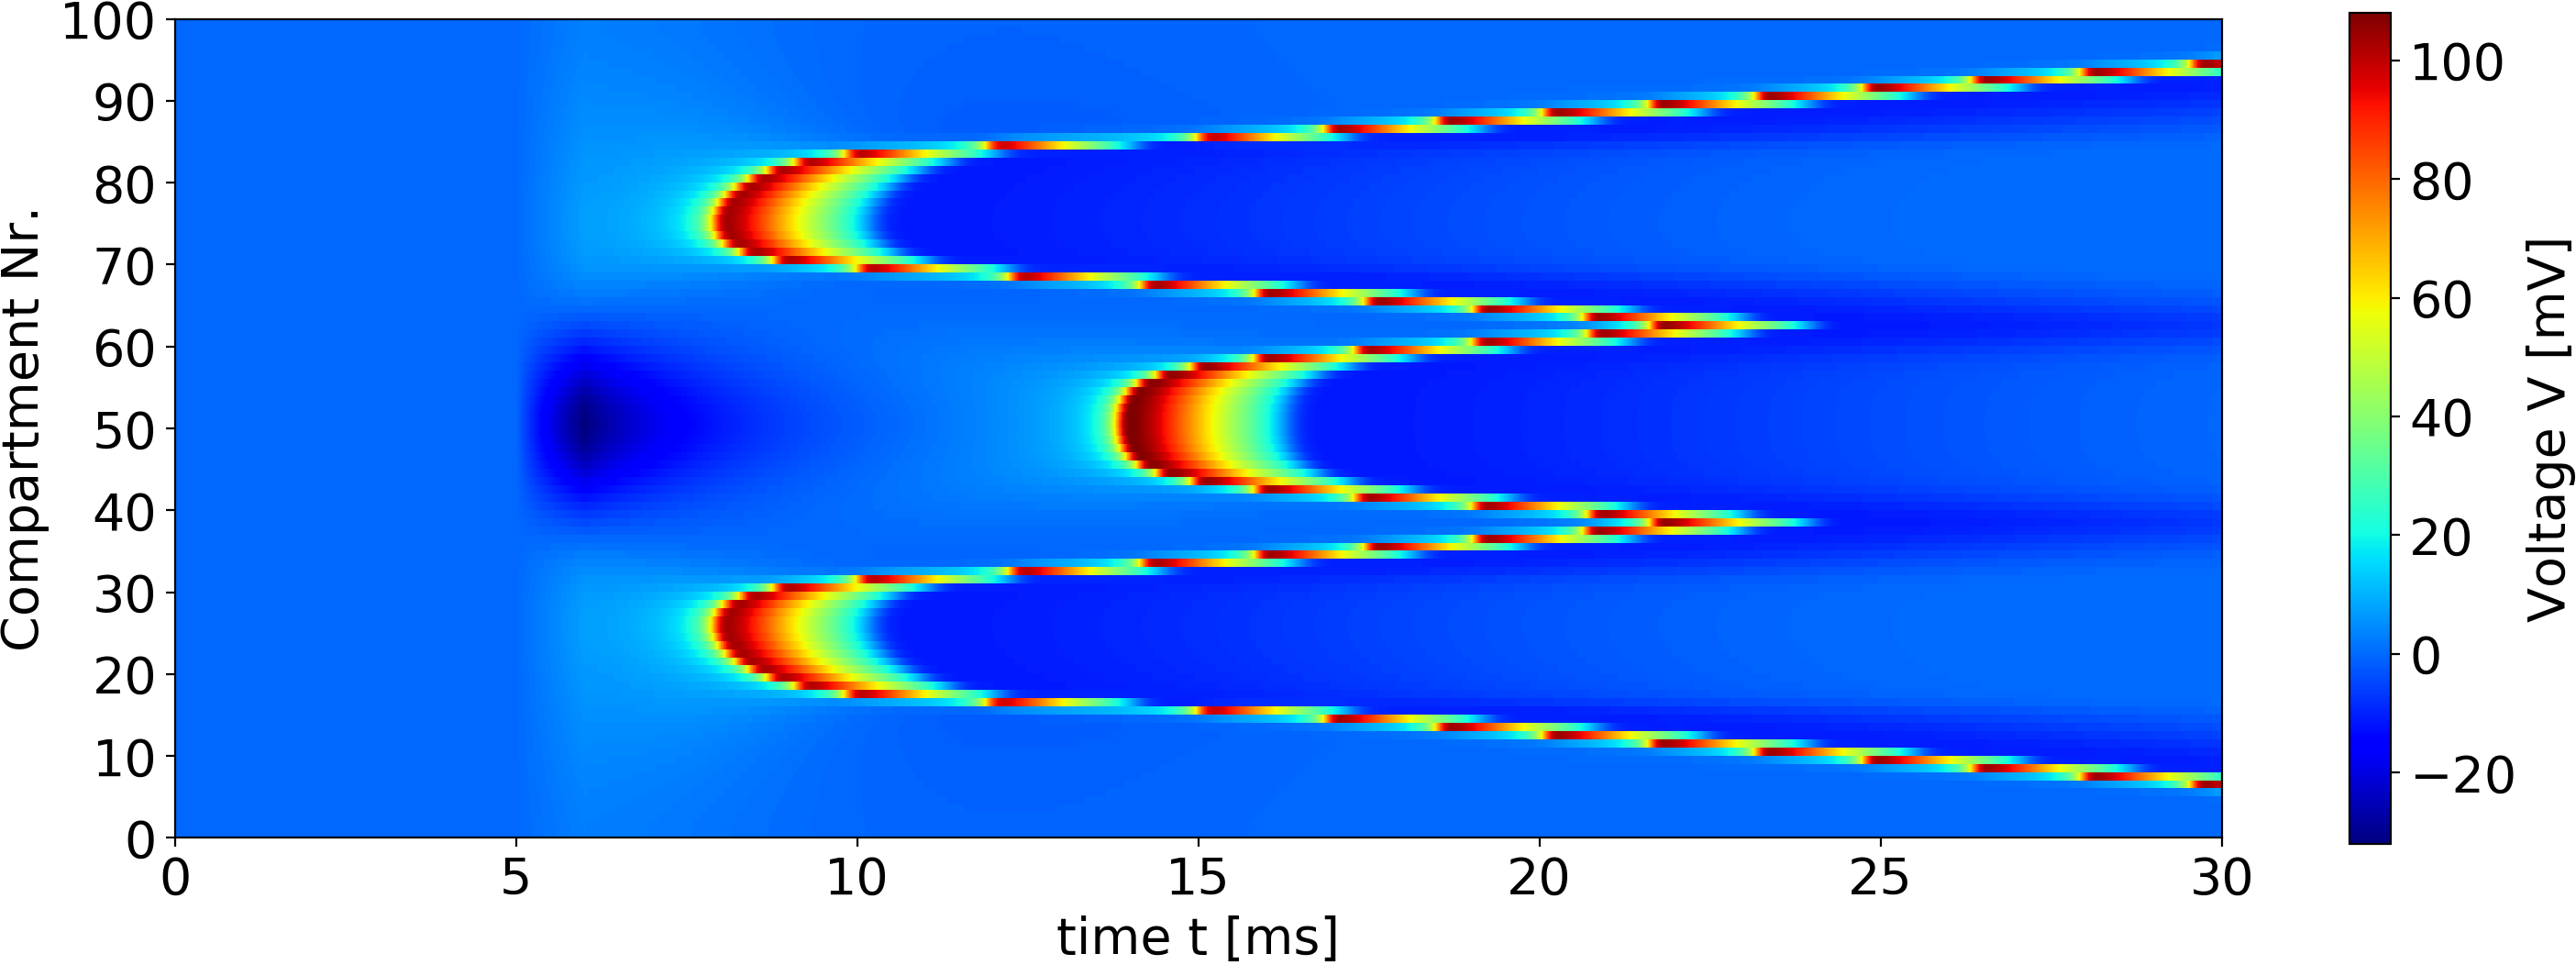
\includegraphics[scale=0.47]{3_6.png}
		\captionsetup{width=\linewidth}  %choose the with of the caption
		\caption{Propagation of the action potential when stimulated at t = 5 ms with a phase duration of 1 ms. Additionally parameter: mono-phasic pulse with 5 mA.}		
		\label{fig36} %choose a label, see subsection references
	\end{flushleft}
\end{figure}


\end{document}
